\fancyhf{}
\setlength{\headheight}{14.49998pt}
\lhead{\textsl{\footnotesize{\nouppercase{\rightmark}}}}
\rhead{\textsl{\footnotesize{\nouppercase{\leftmark}}}}

\cfoot{\thepage}
\rfoot{\textsl{\footnotesize}}

\chapter{General Context}

\section{Introduction}
The global transition toward renewable energy\cite{iea_renewables_2024} has accelerated the demand for accessible, customer-centered solutions in the solar sector. As households and businesses increasingly consider photovoltaic installations\cite{irena_capacity_2024}, companies are challenged not only to offer technically viable products, but also to provide rapid, reliable, and persuasive commercial guidance during the earliest stages of customer contact. In this environment, response speed, communication quality, and availability across digital channels have become decisive competitive factors.

At the same time, customer behavior has shifted toward instant messaging platforms, where users expect immediate answers and seamless interaction. For a solar panel company, this creates a strategic need to engage prospects directly on user facing platforms, while maintaining coherent communication and high informational accuracy. Traditional sales processes, often limited by human availability and delayed follow-up, may reduce conversion opportunities when potential clients do not receive timely preliminary estimates or clear next steps.

This chapter establishes the general context of the project by presenting the market, organizational, and technological motivations that led to the development of an AI-based commercial assistant. It frames the core problem addressed by the project, clarifies its objectives and expected business value, and defines the scope within which the solution was designed. By doing so, it provides the necessary foundation for understanding the architectural, methodological, and implementation decisions discussed in the following chapters.
\section{Company Background}
Sparky is a leading provider of solar panel solutions, committed to making renewable energy accessible and affordable for residential and commercial customers. With a strong focus on innovation and customer satisfaction, Sparky has established itself as a trusted name in the solar industry especially in Sfax. The company offers a wide range of products and services, including solar panel installation, maintenance, and financing options. Sparky's mission is to empower individuals and businesses to transition to clean energy by providing high-quality products and exceptional service. As the demand for solar energy continues to grow, Sparky recognizes the need to enhance its customer engagement strategies and streamline its sales processes to better serve its expanding customer base.

\begin{figure}[htbp]
    \centering
    
\includegraphics[width=0.9\textwidth]{Images/logo_sparky.jpg}
    \caption{Sparky Company Logo.}
    \label{fig:sparky-logo}
\end{figure}

\section{Key Concepts}
This section introduces the fundamental concepts used throughout the project and clarifies the terminology adopted in later chapters. It focuses on the two technical pillars of the solution -- LLM behavior and web integration mechanisms. This way, architectural and implementation choices can be interpreted with the proper context.

\subsection{LLM Concepts}
The LLM Concepts subsection establishes the theoretical foundations required to understand how a modern AI chatbot operates in a real commercial setting. Before analyzing architecture and implementation choices, it is necessary to clarify the core notions that govern LLM behavior, including token-based generation, context dependence, system-level instruction control, and model limitations such as hallucination.

\subsubsection{LLM Definition}
Large Language Models (LLMs) are high-capacity, parameterized probabilistic models designed to estimate the conditional likelihood of linguistic sequences, typically formalized as $(P(x_t \mid x_{<t}))$ , where each token is predicted from its prior context. In contemporary NLP, LLMs are predominantly implemented using Transformer architectures\cite{vaswani2017attention} and trained through self-supervised learning on very large text corpora\cite{brown2020language}, enabling them to acquire broad statistical representations of syntax, semantics, discourse patterns, and world knowledge.

From an academic perspective, an LLM is therefore not a database of fixed answers but a generative inference system: it produces context-dependent outputs by sampling from learned probability distributions. Its practical capabilities—such as instruction following, summarization, reasoning-like behavior, and domain adaptation through prompting—emerge from scale (data, parameters, and compute), optimization objectives, and inference-time conditioning, rather than explicit symbolic programming or task-specific hard-coding.

\begin{figure}[htbp]
    \centering
    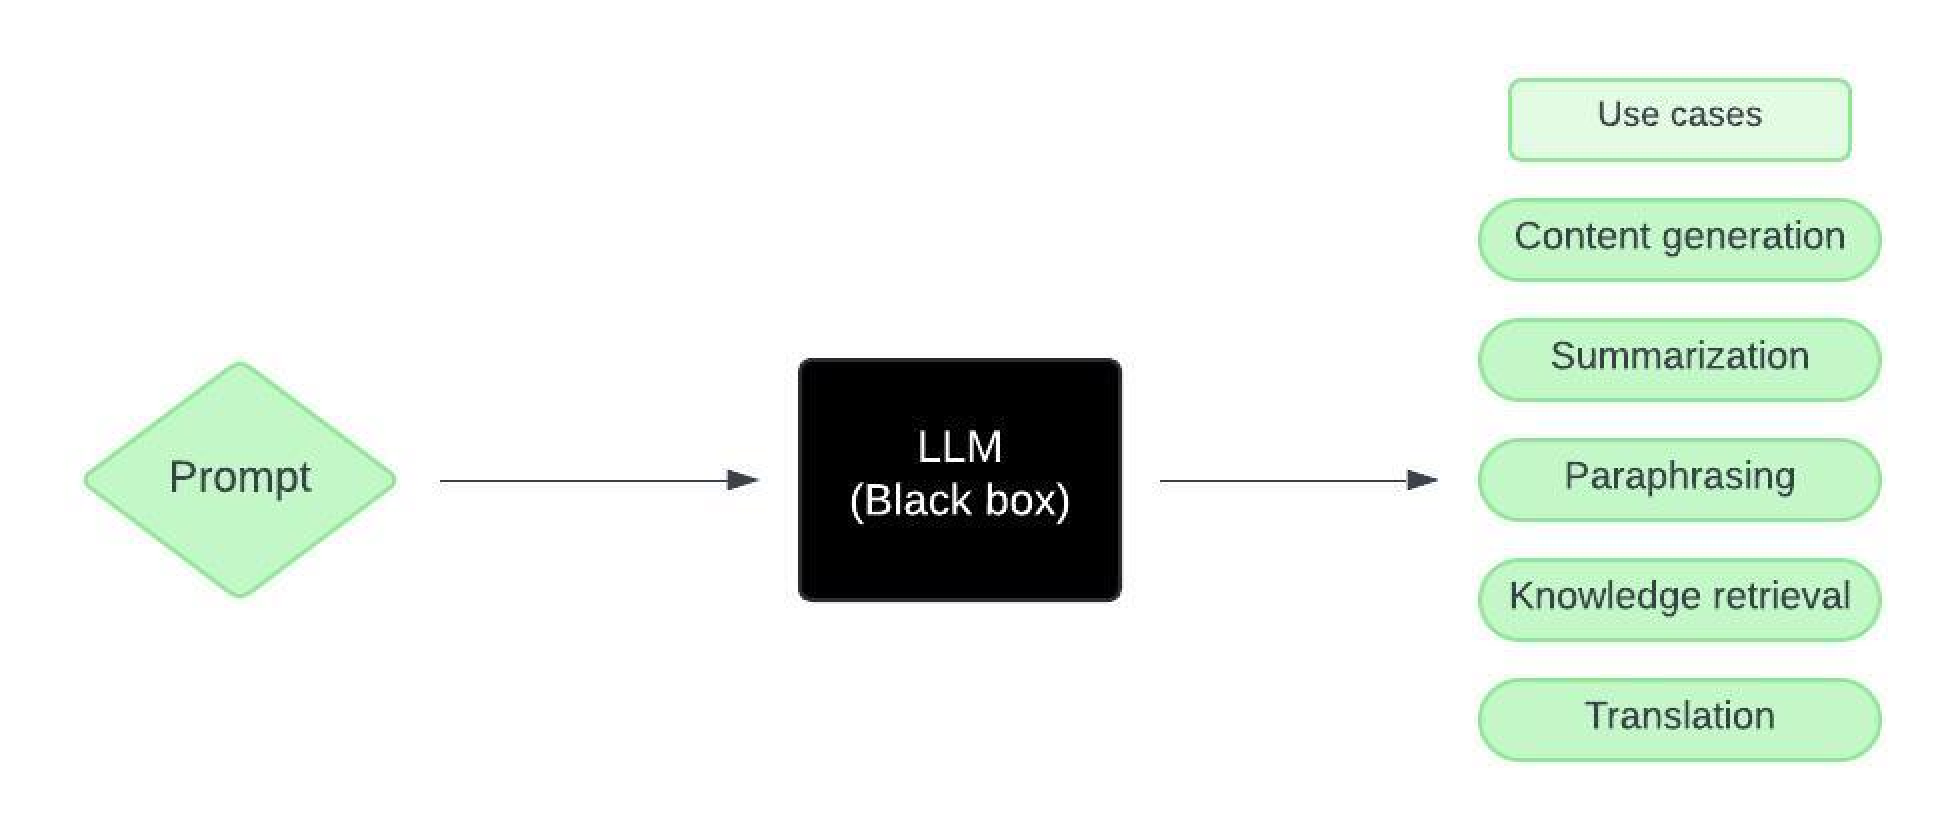
\includegraphics[width=0.9\textwidth]{Images/diagrams/llm_diagram.png}
    \caption{Simplified overview of how an LLM works.}
    \label{fig:llm-diagram}
\end{figure}

\subsubsection{Tokens and Context}
In LLM systems, text is processed as \textit{tokens}, i.e., discrete units produced by a tokenizer. A token may correspond to a full word, a subword, punctuation, or a symbol. Since computation is performed over token sequences rather than raw characters, tokenization directly affects cost, latency, and output quality\cite{sennrich2016bpe}.

\textit{Context} is the ordered token sequence provided to the model at inference time (system instructions, conversation history, and current user input). The model predicts each next token conditionally on this context. Because the context window is finite, relevance management is critical: if important information is omitted, truncated, or buried in noisy history, response reliability decreases.
\subsubsection{Prompt Engineering}
Prompt engineering is the systematic design of model inputs to obtain controlled behavior without modifying model weights. It includes writing precise system instructions, defining role boundaries, specifying response format, and setting decision rules for refusal, escalation, and tool usage\cite{liu2023prompting_survey}.

In applied settings, prompt engineering functions as an operational control layer. It translates business policy into executable linguistic constraints, improves output consistency across sessions, and enables rapid iteration compared with fine-tuning when domain data is limited.
\subsubsection{Hallucination}
Hallucination refers to the generation of content that is linguistically plausible but factually unsupported, incorrect, or not grounded in the available context. This behavior is a known property of probabilistic next-token generation, especially under ambiguity or missing evidence\cite{ji2023hallucination_survey}.

For commercial assistants, hallucination is a high-impact risk because it can produce incorrect technical claims, pricing details, or procedural guidance. Effective mitigation requires grounding mechanisms and explicit uncertainty handling so that the assistant prefers validated outputs or abstention over fabricated precision.

\subsection{Web Concepts}
This subsection introduces the web-layer concepts that structure communication between external messaging platforms and the chatbot backend. These notions provide the technical basis for understanding how events are received, processed, and transmitted in an event-driven integration architecture.
\subsubsection{Webhook Definition}
A webhook is an event-driven HTTP callback through which a platform sends data to a server endpoint when a specific event occurs\cite{github_webhooks_docs}. Instead of repeatedly querying the platform (\textit{polling}), the server receives a push notification containing a structured payload (commonly JSON) with the event metadata and content\cite{meta_webhooks_docs}.

Architecturally, webhooks enable low-latency and resource-efficient integrations between external services and backend systems. In omnichannel messaging, they are the primary mechanism used to transfer incoming user messages from communication platforms to the chatbot server for immediate processing.
\subsubsection{Web SDK Definition}
A Web SDK (Software Development Kit) is a set of libraries, abstractions, and utilities that simplifies interaction with web services and APIs. It typically encapsulates repetitive concerns such as request construction, authentication headers, payload serialization, error mapping, and response parsing\cite{meta_business_sdk_docs}.

Conceptually, an API specifies \textit{what} operations are available, whereas an SDK facilitates \textit{how} those operations are executed in code. In production systems, SDK usage improves implementation consistency, reduces integration errors, and accelerates development compared with manual low-level HTTP handling.

\section{Problem Statement}

Sparky operates in a market where customer demand for solar information is increasing, particularly in Tunisia and, more specifically, in Sfax. Prospective clients frequently initiate contact through social media channels to request service details, technical clarifications, and early price indications before making a purchasing decision.

The company, however, does not have a dedicated social media response team. Commercial staff must divide their time between field operations and digital customer interaction, which creates response delays during high-activity periods. This organizational constraint reduces the company's ability to provide timely first contact at scale.

From a business perspective, delayed replies generate a measurable conversion risk: interested users may lose engagement and redirect their requests to competitors that respond faster. The core problem is therefore the mismatch between growing inquiry volume and available human responsiveness, which directly affects lead retention and commercial opportunity capture.

\section{Existing Solutions}
Before introducing the proposed AI-based approach, it is important to examine the practical alternatives that organizations typically adopt when digital inquiry volume exceeds their immediate response capacity. In similar commercial contexts, three options are frequently considered: expanding internal manpower, outsourcing customer communication to specialized agencies, or deploying rule-based chatbot systems. Reviewing these alternatives clarifies their operational value, but also highlights why they remain only partially adequate for Sparky's specific constraints and objectives.

\subsection{Hiring More Manpower}
One direct solution is to recruit additional staff dedicated to social media interactions. In this model, incoming messages are handled manually by newly assigned agents who provide product information, answer technical questions, and forward qualified leads to the sales team.

In practice, this approach quickly becomes expensive to sustain at scale. Continuous coverage across multiple channels requires recruitment, onboarding, supervision, and recurring payroll costs that may be difficult to absorb for a small or medium-sized company. Service quality can also vary across agents, and response delays may still appear during peak demand.
\subsection{Outsourcing Social Media Management}
Another option is to outsource digital communication to an external agency specialized in customer engagement. This approach can improve response speed without immediately expanding the internal team, while offering predefined workflows and operational reporting.

Although operationally convenient, outsourcing often weakens domain precision and internal alignment. External operators may not fully master technical solar configurations, local installation constraints, or Sparky's quoting practices, which can affect answer quality. It also introduces coordination overhead, stronger dependency on third-party availability, and additional data-governance concerns for customer conversations.
\subsection{Using Rule-Based Chatbots}
Rule-based chatbots represent a third alternative. In this setup, users are guided through predefined question flows, often through clickable buttons for frequent requests. The bot can only answer items explicitly defined in its knowledge tree and returns a fallback response when an input falls outside that scope.

This works well for narrow and repetitive interactions, but commercial conversations are rarely that constrained. Customer messages are often ambiguous, multi-intent, or phrased unpredictably, which rigid menus and scripted trees handle poorly. As coverage expands, maintenance becomes increasingly complex, and the system remains unable to produce contextual reasoning for nuanced quotation scenarios without extensive manual updates.



\section{Proposed Solution}
Our proposed approach is an AI-based commercial assistant deployed on a Node.js Express backend and connected to Facebook Messenger\cite{meta_messenger_platform_docs}, Meta Instagram\cite{meta_instagram_messaging_docs}, and WhatsApp\cite{meta_whatsapp_cloud_api_docs} through dedicated webhook endpoints. Incoming platform events are processed in near real time, enriched with model inference, and returned as channel-compliant responses. Rather than relying on fine-tuning, the system uses a structured system prompt and tool-calling mechanisms to preserve answer consistency and improve factual grounding in quotation-related interactions.

\subsection{Objectives}
This subsection states the operational and business targets that guided the design of the proposed solution.

\subsubsection{Operational Objectives}
The first objective is to provide continuous first-line interaction across the three supported channels through a unified architecture. The assistant must acknowledge messages quickly, maintain coherent multi-turn exchanges, and produce approximate quotation guidance from partial customer inputs. It must also integrate a controlled handoff path so that commercial staff can take over when human intervention is requested.

\subsubsection{Quality and Business Objectives}
The second objective is to improve lead retention by reducing response latency and standardizing informational quality during early customer contact. The assistant should generate policy-aligned outputs, minimize unsupported claims through prompt constraints and tools, and remain maintainable under limited proprietary data availability. In this way, the solution supports commercial conversion while reducing operational pressure on the existing team.


\section{Conclusion}
Chapter 1 established the general context of the project by framing the market dynamics, the company background, and the practical communication challenge created by high inquiry volume and limited response capacity. It also introduced the key technical concepts required for the rest of the report, reviewed common existing alternatives and their trade-offs, and presented the proposed AI-assisted direction with its operational and business objectives.

These elements are essential because they justify both the relevance and the feasibility of the chosen approach before any technical implementation details are examined. The next chapter, \textit{Requirements and Project Scope}, formalizes what the solution must achieve, defines system boundaries, and specifies the constraints that guide design and development decisions.

